\documentclass[a4paper]{article}
\usepackage{graphicx}

\title{Master on Robotics: Exercise 1.1}
\date{18-10-2015}
\author{Juan Pedro Lopez Cabrera}

\begin{document}
  \pagenumbering{gobble}
  \maketitle

  \newpage
  \pagenumbering{arabic}

  \section{Goal}
  Develop a robotic system to point a camera to a ball or face target.
  Two modes of operation:
  \begin{itemize}
    \item Automatic: No human intervention
    \item Teleoperated: with flexi sensors in the hand
  \end{itemize}

  \section{Assignment}
  \begin{enumerate}
    \item Draw a device connection diagram: see Fig. \ref{fig:connections1} in page \pageref{fig:connections1}.
    \item Draw a kinematic frame sketch: see Fig. \ref{fig:kinematics1} in page \pageref{fig:kinematics1}.
    \item Draw a process diagram of the software components involved: see Fig. \ref{fig:process1} in page \pageref{fig:process1}.
    \item Draw a software dependency diagram of the software components involved: see Fig. \ref{fig:dependency1} in page \pageref{fig:dependency1}.
  \end{enumerate}

  \begin{figure}[ht]
    \centering
    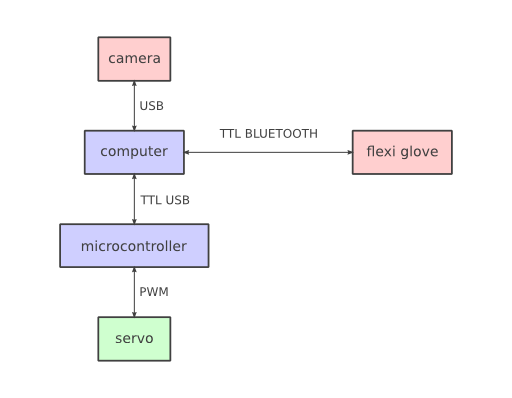
\includegraphics[scale=0.8]{RobocamDeviceConnections}
    \caption{Device connection. The computer-glove communication will occur via BLE link.}
    \label{fig:connections1}
  \end{figure}

  \begin{figure}[ht]
    \centering
    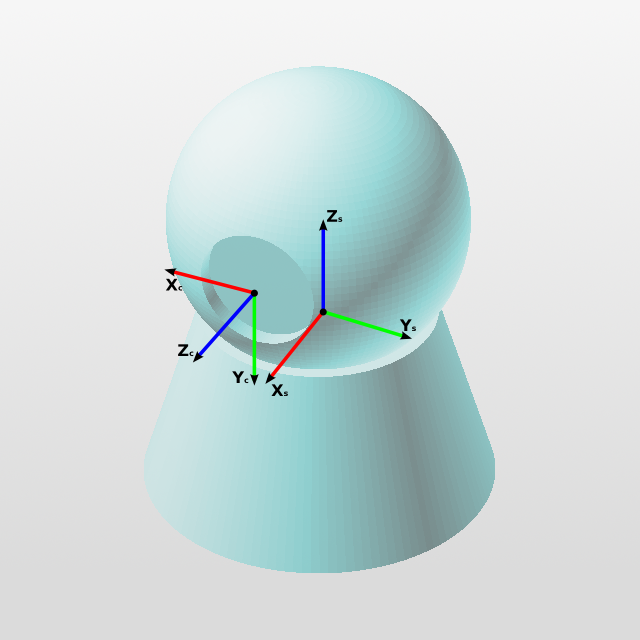
\includegraphics[scale=0.6]{RobocamWithAxes}
    \caption{Kinematic frames for camera and servo. The origin of the camera coordinate system is the optical center of the camera. The servo coordinate system is attached to the base of the head of the robot and its Z axis is in the direction of the servo axis. The servo itself is inside the body of the robot.}
    \label{fig:kinematics1}
  \end{figure}

  \begin{figure}[ht]
    \centering
    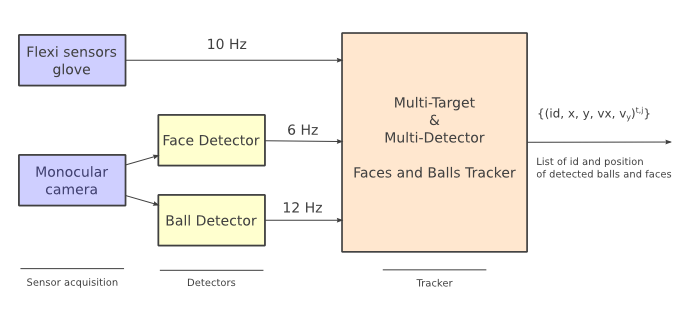
\includegraphics[scale=0.7]{RobocamSoftwareProcess}
    \caption{Software process diagram. The frequency of refresh for detectors is currently an estimate.}
    \label{fig:process1}
  \end{figure}

  \begin{figure}[ht]
    \centering
    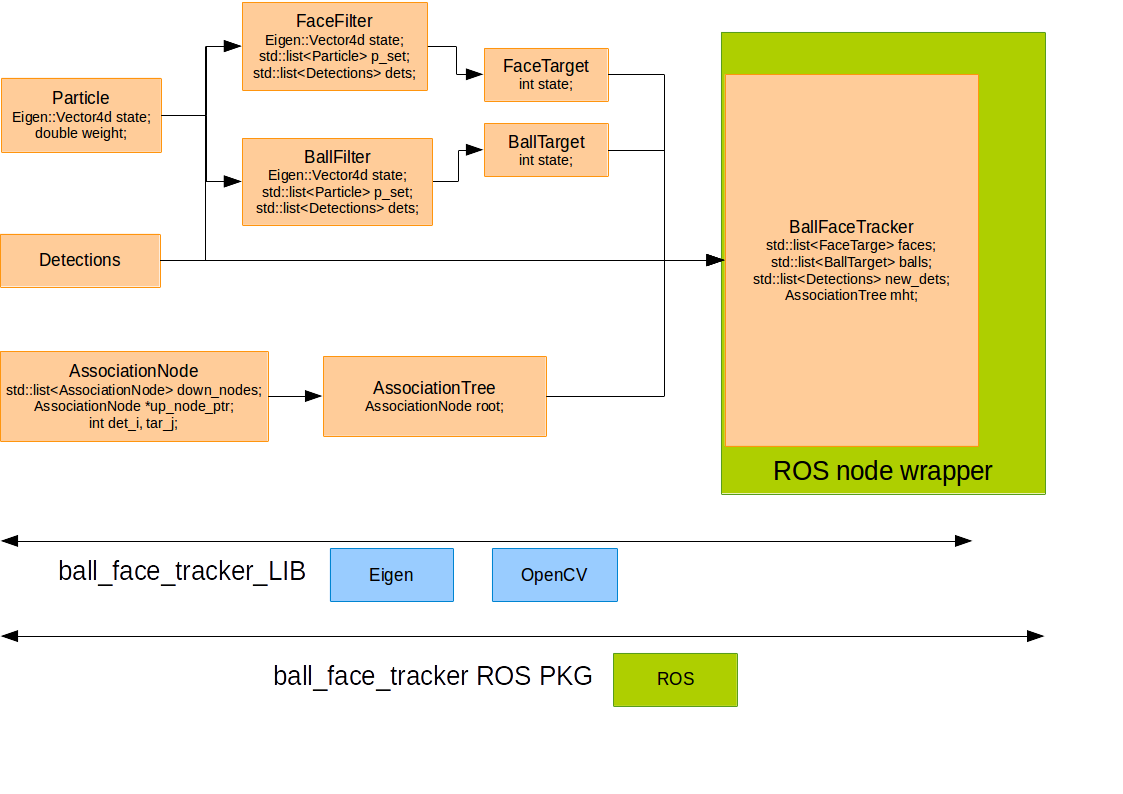
\includegraphics[scale=0.5]{RobocamSoftwareHierarchyDependencies}
    \caption{Software hierarchy and dependencies.}
    \label{fig:dependency1}
  \end{figure}

\end{document}

